%---PACKAGES----------------------------------------
\documentclass[a4paper,11pt]{article}

\usepackage{import}
\import{Packages/}{custom_packages.tex}
\import{Packages/}{custom_macros.tex}

\title{\textbf{Notes on Quiver Gauge Theories}}
\author{Louan Mol\\ \textit{Université Libre de Bruxelles}}
\date{}

% DOCUMENT -----------------------------

\begin{document}

\begin{titlepage}
    
    \maketitle

    \thispagestyle{empty}

    \vspace{2cm}

    \begin{abstract}
        These notes are meant as a work support. The goal is to reproduce and regroup the basics of quiver gauge theories. 
    \end{abstract}

    \vfill

    \hfill Last updated on \today.
    
\end{titlepage}
  
\pagebreak

\tableofcontents

\pagebreak

\nocite{*}

\section{The brane-world paradigm}

    We consider our world to be a slice in the ten-dimensional spacetime of type II superstring theory, i.e. the worldvolume of a D$3$-brane. More precisely, we consider a stack of $n$ D$3$-branes in order to have a $\U(n)$ gauge group. The spacetime is therefore not necessarily $\R^{1,9}$ but of the more general form
    \begin{equation*}
        M = \R^{1,3}\times M^{(6)}.
    \end{equation*}
    This is the so-called \emph{brane-world paradigm}.
    
    Independently from string theory, we can require to have $\mN=1$ supersymmetry in four dimensions. This constrains $M^{(6)}$ to be compact, complex, Kähler and to have $\SU(3)$ holonomy. Namely, $M^{(6)}$ must be a Calabi-Yau threefold. Requireing $\mN=1$ supersymmetry is equivalent too asking that that the configuration resulting from compactification has at least one Killing spinor (covariantly constant spinor). This constant spinor then defines a residual supersymmetry by contracting with the local supersymmetry current. On real $6$-folds, spinors transform under $\SO(6)$. We are therefore looking for the biggest subgroup of $\SO(6)$ that leaves a component of the spinor invariant. In that case the spinor $(1,0,0,0)$ is covariantly conserved, i.e. is a Killing spinor. Using the fact that $\SO(6)\cong\SU(4)$, can clearly see that this subgroup is $\SU(3)$. Our transverse space must therefore have $\SU(3)$ holonomy such that the parallel transport of the spinor $(1,0,0,0)$ under any closed loop is a lower $\SU(3)$ rotation.
    
    If we let the worldvolume of the D$3$-branes carry the requisite gauge theory while the bulk contains gravity, we can relax the compactness condition and study non-compact threefolds. In other words, $M^{(6)}$ is an affine variety that localy models a Calabi-Yau threefold. Intuitively, this can be understood as a Kaluza-Klein compactification where we take the size of the compact dimensions to infinity. The four-dimensional gravity coupling constant being inversely proportional to this quantity, there is no gravity in this limit. This makes the analysis much simpler and therefore also serves as an argument to ignore gravity in the worldvolume theory. Thus far, we have $n$ D$3$-branes on which there is a $\U(n)$ gauge group and transverse to which gravity propagates.

    The only smooth Calabi-Yau threefold is $\C^3$ so we are lead to consider singular Calabi-Yau manifolds or, more precisely, Calabi-Yau orbifolds. We usually denote $S\equiv M^{(6)}$ to remind us of the singular aspect. String theory being a theory of extended objects, it is well-defined on such singularities. We will see that this singular structure of the geometry will break $\U(n)$ into products of gauge groups.
    
    From the point of view of the orbifold, the D$3$-brane is a point. Consequently, there is a crucial relationship between the D$3$-brane worldvolume theory and the Calabi-Yau singularity: the former parametrizes the latter. In other words, the classical vacuum of the gauge theory should be, in explicit coordinates, the defining equation of $S$.

    Mathematically, this brane-world paradigm is the realization of branes as supports of vector bundles (sheaf). Gauge theories on branes are intimately related to algebraic constructions of stable bundles, i.e. holomorphic or algebraic vector bundles that are stable in the sense of geometric invariant theory. In particular, D-brane gauge theories manifest as a natural description of symplectic quotients and their resolutions in geometric invariant theory.

    To summarize in more mathematical terms, our D-branes, together with the stable vector bundle (sheaf) supported thereupon, resolves the transverse Calabi-Yau orbifold which is the vacuum for the gauge theory on the worldvolume as a GIT quotient.

    \begin{result}
        We consider $n$ D$3$-branes carrying a $\U(n)$ gauge group on various orbifolds of $\R^6$. Requiring $\mN=1$ supersymmetry for the worldvolume theory imposes that the transverse space must be a Calabi-Yau orbifold. Ignoring gravity for the worldvolume theory and if we want more interresting cases, we can actually consider the larger class of non-compact singular Calabi-Yau spaces.
    \end{result}
    

\section{The simplest case: $S=\C^3$}

    \subsection{Generalities}

        Let us by studying the simplest configuration were the transverse Calabi-Yau space is non-singular, i.e. it is a proper smooth Calabi-Yau threefold. There actually only when possibility because there is only one smooth Calabi-Yau threefold: $S=\C^3$. In this case, the spacetime is simply flat space $\R^{1,9}=\R^{1,3}\times\R^6$ with a choice a complex structure on $\R^6$. As mentioned above, the worldvolume theory has a $\U(n)$ gauge group. Type IIB superstring theory is a ten-dimensional $\mN=2$ theory so it has $32$ supercharges. The presence of the branes breaks the Lorentz symmetry of $\R^{1,9}$ as
        \begin{equation}
            \SO(1,9)\to\SO(1,3)\times\SO(6),
        \end{equation}
        whereby breaking half of the supersymmetries. We are thus left with $16$ supercharges. In four dimensions, this corresponds to $\mN=4$. The worldvolume theory for $S=\C^3$ is therefore $D=4,\mN=4$ $\U(n)$ SCFT gauge theory. This worldvolume theory, obtained in the non-singular case $S=\C^3$, is called the \emph{parent theory}.

        Note that the D$3$-brane will warp the flat space metric to that of $AdS_5\times S^5$ and the bulk geometry is not strictly $\C^3$. However, as stated above, we are only concerned with the local gauge theory and not with gravitational back-reaction, therefore it suffices to consider $S$ as $\C^3$.

    \subsection{Matter content}

        As discussed in appendix \ref{sec:N4SCFT}, there is only one $D=4,\mN=4$ SCFT theory, up to a choice of gauge group. In our case, we consider the gauge group $G=\U(n)$. The theory has an $\SU(4)_R$ R-symmetry group (transverse rotation group of the D$3$brane) and there are $3n^2$ chiral scalar superfields $\Phi_{IJ}$ and $n^2$ vector superfields. The matter content of this $\mN=4$ gauge theory can be rewritten in terms of $\mN=1$ superfields as follows:
        \begin{equation}
            [\mN = 4 \text{ vector multiplet}] : V = (\lambda_\alpha, A_\mu, D) \oplus \Phi_A = (\phi^A,\psi^A_\alpha,F^A).
        \end{equation}
        with $A=1,2,3$. In other words, after removing the auxiliary fields, the matter content is
        \begin{itemize}
            \item a $\U(n)$ gauge field $A_\mu$ which transforms as a singlets under $\SU(4)_R$.
            \item $4$ Weyl fermions $\psi^{\alpha}$ ($\alpha=1,\dots,4$) that transform under the adjoint of $\U(n)$ and are mixed together under the representation $\boldsymbol{4}$ of $\SU(4)_R$. Each fermion $\psi^\alpha$ is an $n\times n$ matrix and we denote the component by $\psi^{\alpha}_{IJ}$ ($I,J=1,\dots,n$). Explicitely:
            \begin{align}
                \text{Gauge transformation} &: \psi^\alpha \mapsto U \psi^\alpha U^\dagger ,\qquad U\in\U(n),\label{eq:transfpsi1}\\
                \text{R-symmetry} &: \psi^\alpha\mapsto R\indices{^\alpha_\beta}\psi^\beta,\qquad R\in\SU(4)_R.\label{eq:transfpsi2}
            \end{align}
            Note that this gives us $4n^2$ Weyl fermions in total.
            \item $6$ real scalar fields $\phi^{m}_{IJ}$ ($m=1,\dots,6$) transforming under the adjoint representation of $\U(n)$ and under the two-times anti-symmettric representation of $\SU(4)_R$. Each $\phi^m$ is therefore a $n\times n$ matrix with components $\phi^m_{IJ}$. Recall that $\SU(4)\cong\SO(6)$ sithe action of the R-symmetry can be seen as the $\boldsymbol{3}$ of $\SU(3)\subset\SU(4)_R$ acting on three complex scalars or equivalently as the $\boldsymbol{6}$ of $\SO(6)_R$ acting on $6$ real scalars. Explicitely:
            \begin{align}
                \text{Gauge transformation} &= \phi^m \mapsto U \phi^m U^\dagger ,\qquad U\in\U(n),\label{eq:transfphi1}\\
                \text{R-symmetry} &: \phi^m \mapsto R\indices{^m_n}\phi^n,\qquad R\in\SO(6)_R.\label{eq:transfphi2}
            \end{align}
            Note that this gives $6n^2$ real scalars in total. They are the superpartners of the fermions\marker.
        \end{itemize}
        Note that the gauge group $\U(n)$ can also be seen as the group of isometries the metric space $\C^n$ to itself, i.e. $\Hom(\C^n,C^n)$. From this point of view, the transformations \eqref{eq:transfpsi1}-\eqref{eq:transfphi2}can be summarized as
        \begin{align}
            A_\mu&\in\Hom(\C^n,\C^n),\\
            \psi&\in\boldsymbol{4}\otimes\Hom(\C^n,\C^n),\\
            \phi&\in\boldsymbol{6}\otimes\Hom(\C^n,\C^n).
        \end{align}


\section{Projection to daughter theories}

    \subsection{Generalities}

        When the transverse space is singular, the worldvolume theory corresponds to a specific projection of the parent theory that we found in the smooth case $S=\C^3$. We call it the \emph{daughter theory}. This projections depends on the type of singularity that one considers.

        We now wish to pick a discrete group $\Gamma$ and which acts non-trivially on $\R^6$. There are several possibilities:
        \begin{itemize}
            \item $\Gamma\subset(\SU(4)\cong\SO(6))$ naturally acts on $\R^6$. This does not require a choice of complex structure. We get an $\mN=0$ theory.
            \item $\Gamma\subset\SU(3)$ naturally acts on $\C^3$, this also requires a choice of complex structure on $\R^6$. We get an $\mN=1$ theory.
            \item $\Gamma\subset\SU(2)$ naturally acts on the second factor of $\C\times\C^2$, so this requires a choice of complex structure on $\R^6$. We get an $\mN=2$ theory.
        \end{itemize}

        For now, we are interested with $\mN=1$ theories so we consider $\Gamma\subset\SU(3)$ with the action
        \begin{equation}
            \cdot:\left(
            \begin{array}{ccc}
                \Gamma\times\C^3 & \longrightarrow & \C^3 \\
                (\gamma,z) & \longmapsto & \gamma\cdot z
            \end{array}
            \right)
        \end{equation}
        is the representation of $\Gamma$ coming from the fundamental representation of $\SU(3)$, so $\cdot$ is just the matrix product. We can see that the origin is alays a fixed point so this action is never free. Since $\C^3$ is a smooth manifold, this makes $\C^3/\Gamma$ an orbifold. Note this case naturally includes the case $\Gamma\subset\SU(2)$ too, just not the case $\Gamma\in\SO(6)$.

        Note that if $\Gamma$ is a general finite group the condition that $\C^3/\Gamma$ is an Calabi-Yau orbifold means that there must exist a resolution of this orbifold such that the corresponding smooth space is Calabi-Yau, i.e. a crepant resolution. Existence of such a resolution constrains $\Gamma$\marker.

        The prescription is straihgt-forward: we can use the elements $\gamma\in\Gamma$ to project out that states that are not $\Gamma$-invariant. That is, only the the fields such that
        \begin{align}
            \gamma A_\mu \gamma^{-1} &= A_\mu,\label{eq:proj1}\\
            R(\gamma)\gamma \psi_{IJ} \gamma^{-1} &= \psi_{IJ}\label{eq:proj2},\\
            R(\gamma)\gamma \phi_{IJ} \gamma^{-1} &= \phi_{IJ}\label{eq:proj3}
        \end{align}
        are ketp in the spectrum. Note that the fields that transform non-trivially under R-symmetry also have an extra induced action of $\Gamma$. The R-symmetry untouched by $\Gamma$ will be the resulting R-symmetry of daughter theory.

    \subsection{Representation theory realization}

        Let $\{(\rho_i,V_i)\}_{i\in I}$ be a complete set of irreducible representations of $\Gamma$. Since $\Gamma$ is finite, it is particular compact and those representation can be taken to be unitary. Moreover, $i$ takes a finite number of values. Let us consider a representation of $\Gamma$ on $\C^n$, we denote it $(\rho,\C^n)$ and take it unitary. In that case, $\rho(\gamma)\in\U(n)$ and therefore $\rho(\gamma)\omega\rho(\gamma)^{-1}\in\mathfrak{u}(n)$ for any $\omega\in\mathfrak{u}(n)$. In other words, we can construct a representation of $\Gamma$ on $\mathfrak{u}(n)$ from the representation $(\rho,\C^n)$:
        \begin{equation}
            \Ad:\left(
            \begin{array}{ccc}
                \Gamma & \longrightarrow & \GL(\mathfrak{u}(n))) \\
                \gamma & \longmapsto & \Ad_\gamma
            \end{array}
            \right)
        \end{equation}
        with
        \begin{equation}
            \Ad_\gamma:\left(
            \begin{array}{ccc}
                \mathfrak{u}(n) & \longrightarrow & \mathfrak{u}(n) \\
                \omega & \longmapsto & \Ad_\gamma(\omega)\equiv\rho(\gamma)\omega\rho(\gamma)^{-1}
            \end{array}
            \right).
        \end{equation}
        Note that even though this representation looks like the adjoint representation, it is not, because it not on the Lie algebra of $\Gamma$. We use this representation in the expression \eqref{eq:proj1}-\eqref{eq:proj3}.

        We can decompose $(\rho,\C^n)$ as follows:
        \begin{align}
            (\rho,\C^n) &= \bigoplus_{i\in I}~(\rho_i,V_i)^{N_i} \\
            &= \bigoplus_{i\in I}~(\boldsymbol{1}^{N_i}\otimes\rho_i,\C^{N_i}\otimes V_i) \label{eq:decomp:line2}
        \end{align}
        were $N_i$ are integer multiplicities ($(\rho_i,V_i)^{N_i}\equiv(\rho_i,V_i)^{\oplus N_i}$) and $\boldsymbol{1}$ is the trivial representation, so $\Gamma$ acts trivially on the $\C^{N_i}$. We have $\sum_iN_i\dim(\rho_i)=n$. The rewritting \eqref{eq:decomp:line2} will be useful later on.
        
        After the projection, the resulting gauge group is given by the $\Gamma$-invariant part of the gauge group, that is $\Hom(\C^n\C^n)^\Gamma$. That is, we only keep that subspaces of that transform trivially. We use the superscript $\Gamma$ to indicate that we only keep the trivial representations in the decomposition. First, we can see that by Schur lemma \marker
        \begin{equation}
            (V_i\otimes V^*_j)^\Gamma=\delta_{ij}
        \end{equation}
        
        Now since $\Hom(\C^n,\C^n)=\C^n\otimes(\C^n)^*$, we can see that
        \begin{align}
            \Hom(\C^n,\C^n)^\Gamma &= (\C^n\otimes(\C^n)^*)^\Gamma\\
            &= \bigoplus_{i,j\in I} \left((\C^{N_i}\otimes V_i)\otimes(\C^{N_j}\otimes V_j)^*\right)^\Gamma\\
            &= \bigoplus_{i,j\in I} \left(\C^{N_i}\otimes(\C^{N_j})^*\otimes V_i\otimes V^*_j\right)^\Gamma\\
            &= \bigoplus_{i,j\in I} \left(\C^{N_i}\otimes(\C^{N_j})^*\right)^\Gamma\otimes\left(V_i\otimes V^*_j\right)^\Gamma\\
            &= \bigoplus_{i\in I}\C^{N_i}\otimes(\C^{N_i})^*
        \end{align}
        so the daughter gauge group is
        \begin{equation}
            G_{\text{proj}} = \bigotimes_{i\in I}\U(N_i).
        \end{equation}
        Now it turns out that in the low energy effective field theory the $\U(1)$ factor of every $\U(N_i)$ decouples \marker so the resulting gauge group is in fact
        \begin{equation}
            G_{\text{proj}} = \bigotimes_{i\in I}\SU(N_i).
        \end{equation}

        For the matter fields, the reasonning is similar but we now wish to compute $(\mR\otimes\Hom(\C^n,\C^n))^\Gamma$ with $\mR=\boldsymbol{4},\boldsymbol{6}$:
        \begin{align}
            (\mR\otimes\Hom(\C^n,\C^n))^\Gamma &= \bigoplus_{i,j\in I} \left(\mR\otimes (\C^{N_i}\otimes V_i)\otimes(\C^{N_j}\otimes V_j)^*\right)^\Gamma\\
            &= \bigoplus_{i,j\in I} \left(\C^{N_i}\otimes(\C^{N_j})^*\right)^\Gamma\otimes\left(V_i\otimes V^*_j\right)^\Gamma\\
            &= \bigoplus_{i,j\in I}a^\mR_{ij}\left(\C^{N_i}\otimes(\C^{N_j})^*\right)\label{eq:resdecomp}
        \end{align}
        with
        \begin{equation}
            \mR\otimes\rho_i=\bigoplus_{j\in I}a^\mR_{ij}\rho_j\marker.\label{eq:defaij}
        \end{equation}
        Using the orthogonality of characters of irreducible non-equivalent representations, we get that
        \begin{equation}
            a^\mR_{ij} = \frac{1}{\abs{\Gamma}}\sum^r_{\gamma=1} r_\gamma\chi^\mR(\gamma)\chi^i(\gamma)\chi^j(\gamma)^*
        \end{equation}
        where $r_\gamma$ is the order of the conjugacy class containing $\gamma$ and $\chi^i$ is the character of $\rho_i$.

        In the end, we can see that the matter fields become a total of $a^{\boldsymbol{4}}_{ij}$ bi-fundamental fermions and $a^{\boldsymbol{6}}_{ij}$ bi-fundamental bosons transforming as the $(\boldsymbol{\textbf{N}_i},\boldsymbol{\bar{\textbf{N}}_j})$ of $\SU(N_i)\times\SU(N_j)$ under the products of gauge groups.

    \subsection{Field content, quivers and McKay graphs}

        A convenient way the represent the matter content of a daughter theory is to use \emph{quiver diagrams}. A quiver is a finite oriented graph such that each node $i$ represents a gauge factor $\SU(N_i)$ and each arrow $i\to j$ represents a bi-fundamental field transforming under $(\boldsymbol{\textbf{N}_i},\boldsymbol{\bar{\textbf{N}}_j})$. The \emph{adjacency matrix} $A$ of the graph is a $k\times k$ with $k$ being the number of nodes (gauge factors) whose elements $A_{ij}$ are the number of arrows (bi-fundamental fields) from $i$ to $j$. In other words, from \eqref{eq:resdecomp}, the adjacency matrix of the fermions has elements $A_{ij}=a^{\boldsymbol{4}}$ and the one of the scalars has elements $A_{ij}=a^{\boldsymbol{6}}$.

        On the other hand, given finite group $\Gamma$, a representation $(\rho_W,W)$ and a complete set of irreducible representations $\{(\rho_i,V_i)\}_{i\in I}$ of the latter, one can a McKay graph (or quiver) as follows:
        \begin{enumerate}
            \item Draw a vertex for every representation $(\rho_i,V_i)$.
            \item For every representation $(\rho_i,V_i)$, compute the decomposition
            \begin{equation*}
                (\rho_W,V_W)\otimes(\rho_i,V_i)=\bigoplus_j (\rho_j,V_j)^{\oplus n_{ij}}
            \end{equation*}
            where $n_{ij}$ is the multiplicity of $(\rho_j,V_j)$ in the decomposition of $(\rho_W,V_W)\otimes(\rho_i,V_i)$.
            \item For every $n_{ij}>0$, draw $n_{ij}$ arrows from the vertex of $(\rho_i,V_i)$ to the one of $(\rho_j,V_j)$.
        \end{enumerate}
        
        From \eqref{eq:defaij} we see that $n_{ij}=a^{\mR}_{ij}$ and therefore that the matter quivers that we defined previously are exactly the McKay graph associated to the matter representation in question. Or, put differently, the matter content of the daughter theory is encapsulated in the McKay graphs of $\Gamma$ and with respect to $\mR$ with $\mR=\bs{4}$ for spinors and $\mR=\bs{6}$ for scalars. This very important point allows us to use known results on McKay graphs such as the McKay correspondence for example.

    \subsection{$\mN=2$ theories}

        Let us consider that $\Gamma$ is a finite subgroup of $\SU(2)\subset\SU(3)$. It naturally acts on $\C^3$ trough its fundamental representation $\bs{2}$ as $\bs{1}\oplus\bs{2}$ (only acts on 2 coordinates).

    \subsection{$\mN=1$ theories}

    \subsection{String theory realization}

        We discuss a type II theory with a subsector of D$p$-branes for a given $p$ ($p=0,2,4,6,8$ for type IIA and $p=-1,1,3,5,7,9$ for type IIB).

    \subsection{$S=\C^3/\Z_n$}

       Let us consider the representation $(\rho,\C^n)$ of $\Z_n$. A complete set of irreducible representations of $\Z_n$ is given by $\{(\rho_k,V_k)\}_{k=1,\dots,n-1}$ with $V_k=\C$ and
       \begin{equation}
        \rho_i(g)=\zeta^k_n
       \end{equation}
       where $g$ is the generator of $\Z_n$. The representation $(\rho,V)$ can be decomposed as
        \begin{equation}
            (\rho,V)=\bigoplus^{n-1}_{i=0}N_i(\rho_i,V_i).
        \end{equation}
        In other words, it is equivalent to the representation
        \begin{equation}
            \rho(g)=
            \begin{bmatrix}
                1 & & & \cdots & & & 0 \\
                 & \ddots & & & & & \\
                 & & 1 & & & &  \\
                \vdots & & & \ddots & & & \vdots \\
                 & & & & \xi^{n-1}_n & & \\
                 & & & & & \ddots & \\
                0 & & & \cdots & & & \xi^{n-1}_n 
            \end{bmatrix}
            \hspace{-0.2cm}
            \begin{tabular}{l}
            $\left.\lefteqn{\phantom{
                \begin{matrix}
                     a_0\\ \ddots\\ a_0\ 
                \end{matrix} 
            }}\right\}N_0$\\
            \vdots \\
            $\left.\lefteqn{\phantom{
                \begin{matrix}
                    b_0\\ \ddots\\ b_0\ 
                \end{matrix}
            }} \right\}N_{n-1}$
            \end{tabular}.\label{eq:reprrhoZn}
        \end{equation}
        Since $\dim\rho_i=1$, $N\equiv\sum_i N_i = \dim V$. 
        
        The gauge field configurations that are left invariant under the action of $\Z_n$ are therefore the ones that satisfy
        \begin{equation}
            \rho(g)A_\mu\rho(g)^{-1}=A_\mu
        \end{equation}
        for all $g\in\Z_n$. The constrained is easily solved by using the bi-index notation $A_{\mu;i\alpha_i,j\beta_j}$ ($i,j=A,\dots,n-1,\alpha_i,\beta_i=1,\dots,N_i$) for the component of the gauge fields.From \eqref{eq:reprrhoZn}, we can see that
        \begin{equation}
            A_{\mu;i\alpha_i,i\beta_j}\mapsto \rho_i(g)A_{\mu;i\alpha_i,j\beta_j}\rho_j(g)^{-1}=\zeta^{i-j}_nA_{\mu;i\alpha_i,j\beta_j}.
        \end{equation}
        thus only the configurations with $A_{\mu;i\alpha_i,j\beta_j}=0$ if $i\neq j$ are invariant. The gauge field has therefore a block diagonal form:
        \begin{equation}
            A=
            \begin{bmatrix}
                A_{00} & & & \\
                 & A_{11} & & \\
                 & & \ddots & \\
                 & & & 1_{n-1,n-1}
            \end{bmatrix}
        \end{equation}
        with $A_{ij}\equiv (X_{i\alpha_i,j\beta_j})_{\alpha_i=0,\dots,N_i,\beta_j=0,\dots,N_j}$. The block $A_{ii}$ transforms under $\Z_n$ as $(\rho_i,V_i)^{N_i}$.
        Consequently, the gauge group is now broken to
        \begin{equation}
            G_{\text{proj}}=\bigotimes^{n-1}_{i=0}~\U(N_i),
        \end{equation}
        the biggest subgroup of $\U(n)$ that preserves those form of configurations.

        Let us take
        \begin{equation}
            R(g)= \rho^{\oplus n}_0(g) = 
            \begin{bmatrix}
                \xi_n & \cdots & 0 \\
                \cdots & \ddots & \vdots \\
                0 & \cdots & \xi_n
            \end{bmatrix}.
        \end{equation}
        The scalar field configurations that are left invariant satisfy
        \begin{equation}
            R(g)\indices{^m_n}\rho(g)\phi^n\rho(g)^{-1}=\phi^m
        \end{equation}
        for all $g\in\Z_n$. Using bi-index notations, this becomes
        \begin{equation}
            X^m_{i\alpha_i,j\beta_j}\mapsto  \xi_n\delta\indices{^m_n}\rho_i(g) X^n_{i\alpha_i,j\beta_j}\rho_j(g)^{-1} = \xi^{i-j+1}X^m_{i\alpha_i,j\beta_j}
        \end{equation}
        thus only the configurations with $X^n_{i\alpha_i,j\beta_j}=0$ if $i-j+1\neq0$ are left invariant. The scalar fields have a block off-diagonal form:
        \begin{equation}
            X=
            \begin{bmatrix}
                0 & X_{01} & 0 & \cdots & 0 \\
                0 & 0 & X_{12} & \cdots & 0 \\
                & & & \ddots & \\
                X_{n-1,1} & 0 & & \cdots & 0
            \end{bmatrix}
        \end{equation}
        with $X_{ij}\equiv (X_{i\alpha_i,j\beta_j})_{\alpha_i=0,\dots,N_i,\beta_j=0,\dots,N_j}$. The block $X_{ij}$ is an $N_i\times N_j$ block and transforms under the representation $(\boldsymbol{\textbf{N}_i},\boldsymbol{\bar{\textbf{N}}_j})$ of $\U(N_i)\times\U(N_j)$:
        \begin{align*}
            X_{i,i+1} &\in \boldsymbol{\textbf{N}_i}\otimes\boldsymbol{\bar{\textbf{N}}_j} \simeq \Hom(V_{i+1},V_i).
        \end{align*}

        \begin{figure}
            \centering
            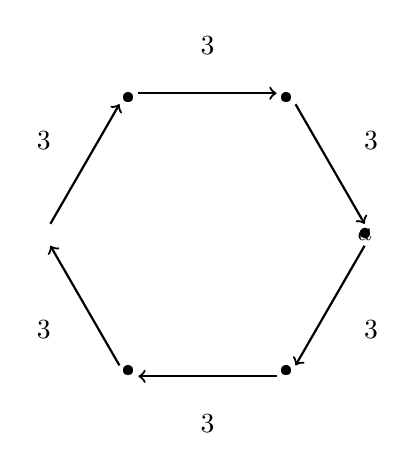
\begin{tikzpicture}
                \foreach \n in {0,...,5}{
                    \draw[->,thick] ({-60*\n-4}:2)--({-60*(\n+1)+4}:2);
                    \draw (30+60*\n:2.4) node{$3$};
                }
                \foreach \n in {-2,-1,0,1,2}{
                    \draw ({-60*\n}:2) node{\textbullet};
                }
                \draw (0:2) node{$a$};
            \end{tikzpicture}
            \caption{Quiver of the $\Z_n$ daughter theory.}
        \end{figure}




        Finally, anomaly cancellation imposes that the number a fields transforming in $\textbf{N}_j$ is equal to the number of fields transforming in $\boldsymbol{\bar{\textbf{N}}}_j$. This results in a constrain on the $N_i$'s:
        \begin{equation}
            \marker .
        \end{equation}
        For $n=2$ or $n=3$ this implies that all $N_i$'s must be equal.

    \subsection{$S=\C\times\C^2/\Z_n$}







    \vspace{5cm}

    \begin{table}[H]
        \centering
        $
        \begin{array}{ccc}
            S & \text{Gauge group} & \text{Matter content} \\ \hline
            \C^3 & \U(n) & \Phi^{\boldsymbol{6}}_{IJ},\Psi^{\boldsymbol{4}}_{IJ} \\
            \C^3/\Z_n & & \\
            \C\times\C^2/\Z_n & & 
        \end{array}
        $
        \caption{Worldvolume theory in terms of $S$.}
    \end{table}


\pagebreak
\appendix

\section{Reminder on $D=4,\mN=4$ super Yang-Mills theory}\label{sec:N4SCFT}
        
    For $D=4,\mN=4$, there is one kind of supermultiplet, the vector multiplet. The decomposition of the $\mN = 4$ vector superfield in terms of $\mN = 1$ representations is as follows:
    \begin{equation}
        [\mN = 4 \text{ vector multiplet}] : V = (\lambda_\alpha, A_\mu, D) \oplus \Phi_A = (\phi^A,\psi^A_\alpha,F^A).
    \end{equation}
    with $A=1,2,3$, i.e. in terms of one vector supermultiplet and three chiral scalar supermultiplets. The propagating degrees of freedom are therefore a vector field, six scalars and four gauginos.
    
    The Lagrangian is very much constrained by $\mN = 4$ supersymmetry. First, the chiral superfields $\Phi^A$ should transform in the adjoint representation of the gauge group $G$, since internal symmetries commute with supersymmetry. This means that all fields transform in the adjoint of $G$.
    
    Moreover, there is a large R-symmetry group, $\SU(4)_R$. The four Weyl fermions transform in the fundamental of $\SU(4)_R$, while the six real scalars in the two times anti-symmetric representation, which is nothing but the fundamental representation of $\SO(6)$. The auxiliary fields are singlets under the R-symmetry group. Using $\mN = 1$ superfield formalism the Lagrangian reads
    \begin{align}
        \begin{split}
            \L^{\mN=4}_{\text{SYM}} &= \frac{1}{32\pi}\Im \left(\tau\int\d^4x\tr(W^\alpha W_\alpha)\right)+\int\d^2\theta\d^2\bar{\theta}\tr\sum^3_{A=1}\bar{\Phi}^Ae^{2gV}\Phi^A\\
            &\quad-\int\d^2\theta\sqrt{2g}\tr\Phi_1[\Phi_2,\Phi_3]+\text{h.c.}
        \end{split}\label{eq:N4lag}
    \end{align}
    where the commutator in the third term appears for the same reason as for the $\mN = 2$ Lagrangian. Notice that the choice of a single $\mN = 1$ supersymmetry generator breaks the full $\SU(4)_R$ R-symmetry to $\SU(3)\times \U(1)_R$. The three chiral superfields transform in the $\boldsymbol{3}$ of $\SU(3)$ and have R-charge $R = 2/3$ under the $\U(1)_R$. It is an easy but tedious exercise to perform the integration in superspace and get an explicit expression in terms of fields. Finally, one can solve for the auxiliary fields and get an expression where only propagating degrees of freedom are present, and where $\SU(4)_R$ invariance is manifest (the fact that the scalar fields transform under the fundamental representation of $\SO(6)$, which is real, makes the R-symmetry group of the $\mN = 4$ theory being at most $\SU(4)$ and not $\U(4)$, in fact).

    As a consequence from the non-renormalization theorems, this theory is conformal.

    \begin{result}
        \textbf{$\boldsymbol{\mN=4}$ Yang-Mills theory.} There is only one $D=4,\mN=4$ Yang-Mills theory and it contains $3$ $\mN=1$ chiral scalar supermutliplet and $1$ $\mN=1$ vector supermultiplet (up to $g$ and $\tau$). This theory is conformal and can be recovered from dimensional reduction of $D=10,\mN=1$ Yang-Mills on $\mathbb{T}^6$.
    \end{result}

\section{The McKay correspondence}

    \subsection{Finite subgroups of $\SL(2,\C)$}

        The first thing to recall is that every finite subgroup of $\SL(2,\C)$ is isomorphic to a subgroup of $\SU(2,\C)$ and vice-versa, so we equivalently talk about the subgroups of $\SU(2)$. The finite subgroups of $\SU(2)$, called the \emph{binary polyhedral groups}, are the doubles covers of the finite subgroups of $\SO(3)$ that are called \emph{polyhedral groups}. They simply constitutes the symmetries of the Platonic solids. The groups fall into two infinite series, associated to the regular polygons, as well as three exceptional, associated with the 5 regular polyhedra: the tetrahedron (self-dual), the cube (and its dual octahedron), the icosahedron (and its dual dodecahedron).

        More precisely, the finite subgroups of $\SU(2)$ are
        \begin{itemize}
            \item $\Z_n$ : cyclic group of order $n$ ($n\geq2$) generated by
            \begin{equation}
                \begin{bmatrix}
                    \zeta_m & 0\\
                    0 & \zeta^{-1}_m
                \end{bmatrix}
            \end{equation}
            \item $2\D_n$ : \emph{binary dihedral groups} of order $4n$ ($n\geq1$) generated by
            \begin{equation}
                A \equiv
                \begin{bmatrix}
                    \zeta_{2m} & 0\\
                    0 & \zeta^{-1}_{2m}
                \end{bmatrix}\quad \text{ and }
                B \equiv 
                \begin{bmatrix}
                    0 & i\\
                    i & 0
                \end{bmatrix}
            \end{equation}
            \item $2\mathcal{T}$ : \emph{binary tetrahedral group} of order $24$ generated by $D_2$ and
            \begin{equation}
                C \equiv \frac{1}{\sqrt{2}}
                \begin{bmatrix}
                    \zeta_8 & \zeta^3_8\\
                    \zeta_8 & \zeta^7_8
                \end{bmatrix}
            \end{equation}
            \item $2\mathcal{O}$ : \emph{binary octahedral group} of order $48$ generated by $\mathcal{T}$ and
            \begin{equation}
                D \equiv 
                \begin{bmatrix}
                    \zeta^3_8 & 0\\
                    0 & \zeta^5_8
                \end{bmatrix}
            \end{equation}
            \item $2\mathcal{I}$ : \emph{binary icosahedral group} of order $120$ generated by
            \begin{equation}
                E \equiv -\frac{1}{\sqrt{5}}
                \begin{bmatrix}
                    \zeta^4_5-\zeta_5 & \zeta^2_5-\zeta^3_5\\
                    \zeta^2_5-\zeta^3_5 & \zeta_5-\zeta^4_5
                \end{bmatrix}\quad \text{ and }
                F \equiv -\frac{1}{\sqrt{5}}
                \begin{bmatrix}
                    \zeta^2_5-\zeta^4_4 & \zeta^4_5-1\\
                    1-\zeta_5 & \zeta^3_5-\zeta_5
                \end{bmatrix}
            \end{equation}
        \end{itemize}
        with $\zeta_m\equiv e^{i\frac{2\pi}{m}}$ such that $(\zeta_m)^m=1$.

        \begin{table}[H]
            \centering
            \begin{tabular}{|c|l|l|l|}
                \hline
                $\Gamma\subset\SU(2)$ & Platonic solids & McKay graph & Variety \\ \hline
                $\Z_n$ &  & \begin{tikzpicture}[baseline={($ (current bounding box.center) - (0,3pt) $)},scale=0.5]
                    \draw (0,0) edge (2*1.25,0);
                    \draw (2*1.25,0) edge[dashed] (3*1.25,0);
                    \draw (3*1.25,0) edge (4*1.25,0);
                    \draw (0,0) edge (2*1.25,-1);
                    \draw (4*1.25,0) edge (2*1.25,-1);
                    \foreach \x in {0,1,2,3,4} {
                        \draw[fill=black] (1.25*\x,0) circle[radius=0.15];
                        \draw (1.25*\x,0) node[above]{$1$};
                    }
                    \draw[fill=black] (1.25*2,-1) circle[radius=0.15];
                    \draw (1.25*2,-1) node[above]{$1$};
                \end{tikzpicture}\quad($n$ nodes) & $z^{n}+xy=0$ \\ \hline
                $2\mathcal{D}_n$ & $n$-polygon & \begin{tikzpicture}[baseline={($ (current bounding box.center) - (0,3pt) $)},scale=0.5]
                    \draw (0,0) edge (2*1.25,0);
                    \draw (2*1.25,0) edge[dashed] (3*1.25,0);
                    \draw (3*1.25,0) edge (4*1.25,0);
                    \draw (4*1.25,0) edge (5*1.25,0);
                    \draw (1.25,0) edge (1.25,-1.25);
                    \draw (4*1.25,0) edge (4*1.25,-1.25);
                    \foreach \x in {0,1,2,3,4,5} {
                        \draw[fill=black] (1.25*\x,0) circle[radius=0.15];
                    }
                    
                    \draw[fill=black] (1.25,-1.25) circle[radius=0.15];
                    \draw (1.25,-1.25) node[right]{$1$};
                    \draw[fill=black] (4*1.25,-1.25) circle[radius=0.15];
                    \draw (4*1.25,-1.25) node[right]{$1$};
                    \draw (0,0) node[above]{$1$};
                    \draw (1.25*5,0) node[above]{$1$};
                    \draw (1.25*1,0) node[above]{$2$};
                    \draw (1.25*2,0) node[above]{$2$};
                    \draw (1.25*3,0) node[above]{$2$};
                    \draw (1.25*4,0) node[above]{$2$};
                \end{tikzpicture}\quad($n+3$ nodes) & $x^2+y^2z+z^{n-1}=0$ \\ \hline
                $2\mathcal{T}$ & tetrahedron & \begin{tikzpicture}[baseline={($ (current bounding box.center) - (0,3pt) $)},scale=0.5]
                    \draw (0,0) edge (4*1.25,0);
                    \draw (2*1.25,0) edge (2*1.25,-2*1.25);
                    \foreach \x in {0,1,2,3,4} {
                        \draw[fill=black] (1.25*\x,0) circle[radius=0.15];
                    }
                    \draw[fill=black] (2*1.25,-1.25) circle[radius=0.15];
                    \draw (2*1.25,-1.25) node[right]{$2$};
                    \draw[fill=black] (2*1.25,-2*1.25) circle[radius=0.15];
                    \draw (2*1.25,-2*1.25) node[right]{$1$};
                    \draw (0,0) node[above]{$1$};
                    \draw (1.25*4,0) node[above]{$1$};
                    \draw (1.25*1,0) node[above]{$2$};
                    \draw (1.25*2,0) node[above]{$3$};
                    \draw (1.25*3,0) node[above]{$2$};
                \end{tikzpicture}\quad($7$ nodes) & $x^2+y^3+z^4=0$ \\ \hline
                $2\mathcal{O}$  & \begin{tabular}{@{}l@{}}cube \\ octahedron\end{tabular} & \begin{tikzpicture}[baseline={($ (current bounding box.center) - (0,3pt) $)},scale=0.5]
                    \draw (0,0) edge (6*1.25,0);
                    \draw (3*1.25,0) edge (3*1.25,-1.25);
                    \foreach \x in {0,1,2,3,4,5,6} {
                        \draw[fill=black] (1.25*\x,0) circle[radius=0.15];
                    }
                    \draw[fill=black] (3*1.25,-1.25) circle[radius=0.15];
                    \draw (3*1.25,-1.25) node[right]{$2$};
                    \draw (0,0) node[above]{$1$};
                    \draw (1.25*1,0) node[above]{$2$};
                    \draw (1.25*2,0) node[above]{$3$};
                    \draw (1.25*3,0) node[above]{$4$};
                    \draw (1.25*4,0) node[above]{$3$};
                    \draw (1.25*5,0) node[above]{$2$};
                    \draw (1.25*6,0) node[above]{$1$};
                \end{tikzpicture}\quad($8$ nodes) & $x^2+y^3+yz^3=0$ \\ \hline
                $2\mathcal{I}$  & \begin{tabular}{@{}l@{}}icosahedron \\ dodecahedron\end{tabular} & \begin{tikzpicture}[baseline={($ (current bounding box.center) - (0,3pt) $)},scale=0.5]
                    \draw (0,0) edge (7*1.25,0);
                    \draw (2*1.25,0) edge (2*1.25,-1.25);
                    \foreach \x in {0,1,2,3,4,5,6,7} {
                        \draw[fill=black] (1.25*\x,0) circle[radius=0.15];
                    }
                    \draw[fill=black] (2*1.25,-1.25) circle[radius=0.15];
                    \draw (2*1.25,-1.25) node[right]{$3$};
                    \draw (0,0) node[above]{$2$};
                    \draw (1.25*1,0) node[above]{$4$};
                    \draw (1.25*2,0) node[above]{$6$};
                    \draw (1.25*3,0) node[above]{$5$};
                    \draw (1.25*4,0) node[above]{$4$};
                    \draw (1.25*5,0) node[above]{$3$};
                    \draw (1.25*6,0) node[above]{$2$};
                    \draw (1.25*7,0) node[above]{$1$};
                \end{tikzpicture}\quad($9$ nodes) & $x^2+y^3+z^5=0$ \\ \hline
            \end{tabular}
            \caption{Binary polyhedral groups and their McKay graphs.Labels over the vertices are the dimension of the representation. We erase the arrow ends if they go in both directions and erase the label if it is
            equal to $1$.}
        \end{table}

    \subsection{Simple Lie algebras}

        \begin{figure}[H]
            \centering
            \begin{tabular}{|c|c|l|}
                \hline
                \begin{tabular}{@{}c@{}}Simple \\ Lie algebra\end{tabular} & Simply laced & \begin{tabular}{@{}l@{}}Dynkin diagram \\ Extended Dybkin diagram\end{tabular} \\ \hline
                $\mathfrak{sl}(n+1,\C),n\geq1$ & yes & 
                \begin{tabular}{@{}l@{}} $A_n:\quad$ \begin{tikzpicture}[baseline={($ (current bounding box.center) - (0,3pt) $)},scale=0.5]
                    \draw (0,0) edge (2*1.25,0);
                    \draw (2*1.25,0) edge[dashed] (3*1.25,0);
                    \draw (3*1.25,0) edge (4*1.25,0);
                    \foreach \x in {0,1,2,3,4} {
                    \draw[fill=white] (1.25*\x,0) circle[radius=0.15];
                    }
                    \end{tikzpicture}\quad($n$ nodes) \\[0.4cm] $\tilde{A}_n:\quad$ \begin{tikzpicture}[baseline={($ (current bounding box.center) - (0,3pt) $)},scale=0.5]
                        \draw (0,0) edge (2*1.25,0);
                        \draw (2*1.25,0) edge[dashed] (3*1.25,0);
                        \draw (3*1.25,0) edge (4*1.25,0);
                        \draw (0,0) edge (2*1.25,1);
                        \draw (4*1.25,0) edge (2*1.25,1);
                        \foreach \x in {0,1,2,3,4} {
                            \draw[fill=white] (1.25*\x,0) circle[radius=0.15];
                        }
                        \draw[fill=black] (1.25*2,1) circle[radius=0.15];
                    \end{tikzpicture}\quad($n+1$ nodes)\end{tabular} \\ \hline
                $\mathfrak{so}(2n+1,\R),n\geq2$ & no & 
                \begin{tabular}{@{}l@{}}$B_n:\quad$ \begin{tikzpicture}[baseline={($ (current bounding box.center) - (0,3pt) $)},scale=0.5]
                    \draw (0,0) edge (2*1.25,0);
                    \draw (2*1.25,0) edge[dashed] (3*1.25,0);
                    \draw (3*1.25+0.65-0.15,0.21) -- (3*1.25+0.65+0.15,0) -- (3*1.25+0.65-0.15,-0.21);
                    \draw (3*1.25,0.07) -- (4*1.25,0.07);
                    \draw (3*1.25,-0.07) -- (4*1.25,-0.07); 
                    \foreach \x in {0,1,2,3,4} {
                    \draw[fill=white] (1.25*\x,0) circle[radius=0.15];
                    }
                    \end{tikzpicture}\quad (\marker nodes) \\[0.4cm] $\tilde{B}_n:\quad$ \begin{tikzpicture}[baseline={($ (current bounding box.center) - (0,3pt) $)},scale=0.5]
                        \draw (1.25,0) edge (2*1.25,0);
                        \draw (0,0.7) edge (1.25,0);
                        \draw (0,-0.7) edge (1.25,0);
                        \draw (2*1.25,0) edge[dashed] (3*1.25,0);
                        \draw (3*1.25+0.65-0.15,0.21) -- (3*1.25+0.65+0.15,0) -- (3*1.25+0.65-0.15,-0.21);
                        \draw (3*1.25,0.07) -- (4*1.25,0.07);
                        \draw (3*1.25,-0.07) -- (4*1.25,-0.07); 
                        \foreach \x in {1,2,3,4} {
                            \draw[fill=white] (1.25*\x,0) circle[radius=0.15];
                        }
                        \draw[fill=white] (0,0.7) circle[radius=0.15];
                        \draw[fill=black] (0,-0.7) circle[radius=0.15];
                    \end{tikzpicture}\quad(\marker nodes)\end{tabular} \\ \hline
                $\mathfrak{sp}(2n,\C),n\geq3$ & no & 
                \begin{tabular}{@{}l@{}}$C_n:\quad$ \begin{tikzpicture}[baseline={($ (current bounding box.center) - (0,4pt) $)},scale=0.5]
                    \draw (0,0) edge (2*1.25,0);
                    \draw (2*1.25,0) edge[dashed] (3*1.25,0);
                    \draw (3*1.25+0.65+0.15,0.21) -- (3*1.25+0.65-0.15,0) -- (3*1.25+0.65+0.15,-0.21);
                    \draw (3*1.25,0.07) -- (4*1.25,0.07);
                    \draw (3*1.25,-0.07) -- (4*1.25,-0.07); 
                    \foreach \x in {0,1,2,3,4} {
                    \draw[fill=white] (1.25*\x,0) circle[radius=0.15];
                    }
                    \end{tikzpicture}\quad (\marker nodes) \\[0.4cm] $\tilde{C}_n:\quad$ \begin{tikzpicture}[baseline={($ (current bounding box.center) - (0,4pt) $)},scale=0.5]
                        \draw (0.65-0.15,0.21) -- (0.65+0.15,0) -- (0.65-0.15,-0.21);
                        \draw (0,0.07) -- (1.25,0.07);
                        \draw (0,-0.07) -- (1.25,-0.07);
                        \draw (1.25,0) edge (2*1.25,0);
                        \draw (2*1.25,0) edge[dashed] (3*1.25,0);
                        \draw (3*1.25+0.65+0.15,0.21) -- (3*1.25+0.65-0.15,0) -- (3*1.25+0.65+0.15,-0.21);
                        \draw (3*1.25,0.07) -- (4*1.25,0.07);
                        \draw (3*1.25,-0.07) -- (4*1.25,-0.07); 
                        \foreach \x in {1,2,3,4} {
                            \draw[fill=white] (1.25*\x,0) circle[radius=0.15];
                        }
                        \draw[fill=black] (0,0) circle[radius=0.15];
                    \end{tikzpicture}\quad(\marker nodes)\end{tabular} \\ \hline
                $\mathfrak{so}(2n,\R),n\geq4$ & yes &
                \begin{tabular}{@{}l@{}}$D_n:\quad$ \begin{tikzpicture}[baseline={($ (current bounding box.center) - (0,3pt) $)},scale=0.5]
                    \draw (0,0) edge (2*1.25,0);
                    \draw (2*1.25,0) edge[dashed] (3*1.25,0);
                    \draw (3*1.25,0) -- (4*1.25,0.7);
                    \draw (3*1.25,0) -- (4*1.25,-0.7); 
                    \foreach \x in {0,1,2,3} {
                    \draw[fill=white] (1.25*\x,0) circle[radius=0.15];
                    }
                    \draw[fill=white] (1.25*4,0.7) circle[radius=0.15];
                    \draw[fill=white] (1.25*4,-0.7) circle[radius=0.15];
                    \end{tikzpicture}\quad($n$ nodes) \\[0.4cm] $\tilde{D}_n:\quad$  \begin{tikzpicture}[baseline={($ (current bounding box.center) - (0,3pt) $)},scale=0.5]
                        \draw (0,0.7) edge (1.25,0);
                        \draw (0,-0.7) edge (1.25,0);
                        \draw (1.25,0) edge (2*1.25,0);
                        \draw (2*1.25,0) edge[dashed] (3*1.25,0);
                        \draw (3*1.25,0) -- (4*1.25,0.7);
                        \draw (3*1.25,0) -- (4*1.25,-0.7); 
                        \foreach \x in {1,2,3} {
                            \draw[fill=white] (1.25*\x,0) circle[radius=0.15];
                        }
                        \draw[fill=white] (0,0.7) circle[radius=0.15];
                        \draw[fill=black] (0,-0.7) circle[radius=0.15];
                        \draw[fill=white] (1.25*4,0.7) circle[radius=0.15];
                        \draw[fill=white] (1.25*4,-0.7) circle[radius=0.15];
                    \end{tikzpicture}\quad(\marker nodes)\end{tabular} \\ \hline
                $\mathfrak{e}_6$ & yes &
                \begin{tabular}{@{}l@{}}$E_6:\quad$ \begin{tikzpicture}[baseline={($ (current bounding box.south) + (0,1pt) $)},scale=0.5]
                    \draw (0,0) edge (4*1.25,0);
                    \draw (2*1.25,0) edge (2*1.25,1.25);
                    \foreach \x in {0,1,2,3,4} {
                    \draw[fill=white] (1.25*\x,0) circle[radius=0.15];
                    }
                    \draw[fill=white] (2*1.25,1.25) circle[radius=0.15];
                    \end{tikzpicture} \quad($6$ nodes) \\[0.4cm]  $\tilde{E}_6:\quad$ \begin{tikzpicture}[baseline={($ (current bounding box.south) + (0,1pt) $)},scale=0.5]
                        \draw (0,0) edge (4*1.25,0);
                        \draw (2*1.25,0) edge (2*1.25,2*1.25);
                        \foreach \x in {0,1,2,3,4} {
                            \draw[fill=white] (1.25*\x,0) circle[radius=0.15];
                        }
                        \draw[fill=white] (2*1.25,1.25) circle[radius=0.15];
                        \draw[fill=black] (2*1.25,2*1.25) circle[radius=0.15];
                    \end{tikzpicture}\quad($6$ nodes)\end{tabular} \\ \hline
                $\mathfrak{e}_7$ & yes & 
                \begin{tabular}{@{}l@{}} $E_7:\quad$ \begin{tikzpicture}[baseline={($ (current bounding box.south) + (0,1pt) $)},scale=0.5]
                    \draw (0,0) edge (5*1.25,0);
                    \draw (2*1.25,0) edge (2*1.25,1.25);
                    \foreach \x in {0,1,2,3,4,5} {
                    \draw[fill=white] (1.25*\x,0) circle[radius=0.15];
                    }
                    \draw[fill=white] (2*1.25,1.25) circle[radius=0.15];
                    \end{tikzpicture} \quad($7$ nodes) \\[0.4cm] $\tilde{E}_7:\quad$ \begin{tikzpicture}[baseline={($ (current bounding box.south) + (0,1pt) $)},scale=0.5]
                        \draw (-1.25,0) edge (5*1.25,0);
                        \draw (2*1.25,0) edge (2*1.25,1.25);
                        \foreach \x in {0,1,2,3,4,5} {
                            \draw[fill=white] (1.25*\x,0) circle[radius=0.15];
                        }
                        \draw[fill=black] (-1.25,0) circle[radius=0.15];
                        \draw[fill=white] (2*1.25,1.25) circle[radius=0.15];
                    \end{tikzpicture}\quad($8$ nodes)\end{tabular} \\ \hline
                $\mathfrak{e}_8$ & yes & 
                \begin{tabular}{@{}l@{}}$E_8:\quad$ \begin{tikzpicture}[baseline={($ (current bounding box.south) + (0,1pt) $)},scale=0.5]
                    \draw (0,0) edge (6*1.25,0);
                    \draw (2*1.25,0) edge (2*1.25,1.25);
                    \foreach \x in {0,1,2,3,4,5,6} {
                    \draw[fill=white] (1.25*\x,0) circle[radius=0.15];
                    }
                    \draw[fill=white] (2*1.25,1.25) circle[radius=0.15];
                    \end{tikzpicture} \quad($8$ nodes) \\[0.4cm] $\tilde{E}_8:\quad$ \begin{tikzpicture}[baseline={($ (current bounding box.south) + (0,1pt) $)},scale=0.5]
                        \draw (0,0) edge (7*1.25,0);
                        \draw (2*1.25,0) edge (2*1.25,1.25);
                        \foreach \x in {0,1,2,3,4,5,6} {
                            \draw[fill=white] (1.25*\x,0) circle[radius=0.15];
                        }
                        \draw[fill=black] (7*1.25,0) circle[radius=0.15];
                        \draw[fill=white] (2*1.25,1.25) circle[radius=0.15];
                    \end{tikzpicture}\quad($9$ nodes)\end{tabular} \\ \hline
                $\mathfrak{f}_4$ & no & 
                \begin{tabular}{@{}l@{}}$F_4:\quad$ \begin{tikzpicture}[baseline={($ (current bounding box.center) - (0,3pt) $)},scale=0.5]
                    \draw (0,0) edge (1.25,0);
                    \draw (2*1.25,0) edge (3*1.25,0);
                    \draw (1*1.25+0.65-0.15,0.21) -- (1*1.25+0.65+0.15,0) -- (1*1.25+0.65-0.15,-0.21);
                    \draw (1*1.25,0.07) -- (2*1.25,0.07);
                    \draw (1*1.25,-0.07) -- (2*1.25,-0.07); 
                    \foreach \x in {0,1,2,3} {
                    \draw[fill=white] (1.25*\x,0) circle[radius=0.15];
                    }
                    \end{tikzpicture} \quad($4$ nodes) \\[0.4cm] $\tilde{F}_4:\quad$  \begin{tikzpicture}[baseline={($ (current bounding box.center) - (0,3pt) $)},scale=0.5]
                        \draw (-1.25,0) edge (1.25,0);
                        \draw (2*1.25,0) edge (3*1.25,0);
                        \draw (1*1.25+0.65-0.15,0.21) -- (1*1.25+0.65+0.15,0) -- (1*1.25+0.65-0.15,-0.21);
                        \draw (1*1.25,0.07) -- (2*1.25,0.07);
                        \draw (1*1.25,-0.07) -- (2*1.25,-0.07); 
                        \foreach \x in {0,1,2,3} {
                            \draw[fill=white] (1.25*\x,0) circle[radius=0.15];
                        }
                        \draw[fill=black] (-1.25,0) circle[radius=0.15];
                    \end{tikzpicture}\quad($5$ nodes)\end{tabular} \\ \hline
                $\mathfrak{g}_2$ & no & 
                \begin{tabular}{@{}l@{}} $G_2:\quad$  \begin{tikzpicture}[baseline={($ (current bounding box.center) - (0,3pt) $)},scale=0.5]
                    \draw (0,0) edge (1.25,0);
                    \draw (0.65-0.15,0.21) -- (0.65+0.15,0) -- (0.65-0.15,-0.21);
                    \draw (0,0.11) -- (1.25,0.11);
                    \draw (0,-0.11) -- (1.25,-0.11); 
                    \foreach \x in {0,1} {
                    \draw[fill=white] (1.25*\x,0) circle[radius=0.15];
                    }
                    \end{tikzpicture} \quad($2$ nodes) \\[0.4cm] $\tilde{G}_2:\quad$ \begin{tikzpicture}[baseline={($ (current bounding box.center) - (0,3pt) $)},scale=0.5]
                        \draw (-1.25,0) edge (1.25,0);
                        \draw (0.65-0.15,0.21) -- (0.65+0.15,0) -- (0.65-0.15,-0.21);
                        \draw (0,0.11) -- (1.25,0.11);
                        \draw (0,-0.11) -- (1.25,-0.11); 
                        \foreach \x in {0,1} {
                            \draw[fill=white] (1.25*\x,0) circle[radius=0.15];
                        }
                        \draw[fill=black] (-1.25,0) circle[radius=0.15];
                    \end{tikzpicture}\quad($3$ nodes)\end{tabular} \\ \hline
            \end{tabular}
            \caption{Simple Lie algebras and their (extended) Dynkin diagrams.}
        \end{figure}

    \subsection{Classical McKay correspondence}

    \subsection{Geometrical McKay correspondence}

\section{Calabi-Yau manifolds, orbifolds and crepant resolutions}

    Simply put, a \emph{Calabi-Yau manifold} is a Kähler manifold with trivial canonical bundle or, equivalently, with a Kähler metric whose global holonomy is contained in $\SU(n)$. This is equivalent to having a trivial canonical bundle.

    A \emph{Calabi-Yau orbifold} is the quotient of a smooth Calabi-Yau manifold by a discrete group action which generically has fixed points. From a algebraic geometry perspective we can try to resolve the orbifold singularity. A resolution $(X,\pi)$ of $\C^n/\Gamma$ is a non-singular complex manifold $X$ of dimension $n$ with a proper biholomorphic map 
    \begin{equation}
        \pi:X\to\C^n/\Gamma
    \end{equation}
    that induces a biholomorphism between dense open sets. A resolution $(X,\pi)$ of $\C^n/\Gamma$ is called a \emph{crepant resolution}\index{resolution!crepant}\footnote{For a resolution of singularities we can define a notion of discrepancy. A crepant resolution is a resolution
        without discrepancy.} if the canonical bundles of $X$ and $\C^n/\Gamma$ are isomorphic, i.e.
        \begin{equation*}
            K_X\cong\pi^*(K_{\C^n/\Gamma}).
        \end{equation*}
    Since Calabi-Yau manifolds have trivial canonical bundle, to obtain a Calabi-Yau structure on $X$ one must choose a crepant resolutions of singularities.

    It turns out that the amount of information we know about a crepant resolution of singularities of $\C^n/\Gamma$ depends dramatically on the dimension $n$ of the orbifold:
    \begin{itemize}
        \item $n=2$: a crepant always exists and is unique. Its topology is entirely described in terms of the finite group $\Gamma$ (via the McKay correspondence).
        \item $n=3$: a crepant resolution always exists but it is not unique; they are related by flops. However all the crepant resolutions have the same Euler and Betti numbers: the \emph{stringy} Betti and Hodge numbers of the orbifold.
        \item $n\geq4$: very little is known; crepant resolution ecists in rather special cases. Many singularity are terminal, which implies that they admit no crepant resolution.
    \end{itemize}

    

\pagebreak

\listofmarker
\addcontentsline{toc}{chapter}{\listmarkername}

\pagebreak

\printbibliography

\end{document}